\begin{frame}
  \frametitle{\problemtitle}
  \begin{block}{Problem}
    There is a game board with $n$ holes, initially hole $i$ contains $a_i$ stones.
    Perform the following ''game`` exactly $t$ times:
    Drop one stone into hole $1$ and simulate according to the rules of Congklak.
    How many stones are in each hole after playing $t$ of those games?
  \end{block}
  \begin{center}
    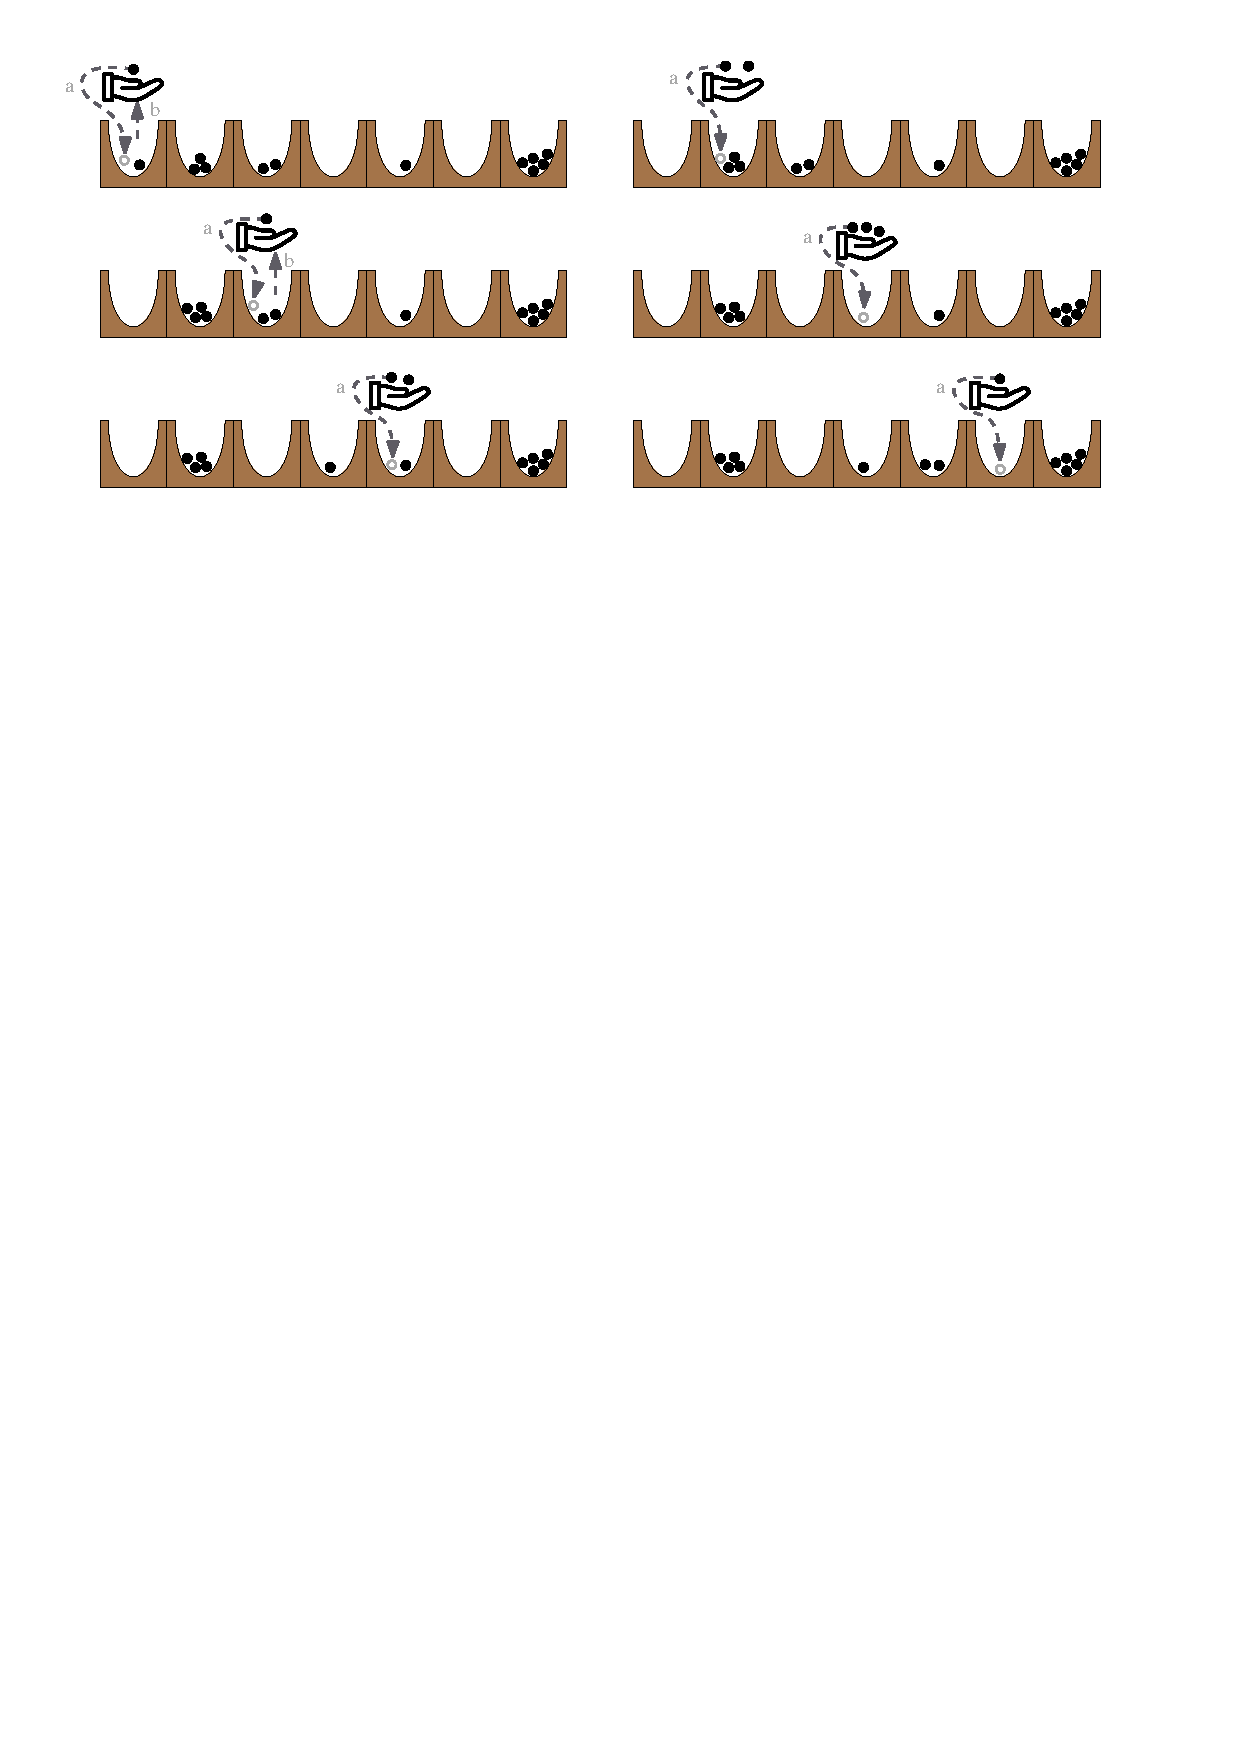
\includegraphics[width = .8\textwidth]{solution-vis.pdf}
  \end{center}
\end{frame}

\newcommand{\cMark}[1]{\textbf{\textcolor{blue}{#1}}}

\begin{frame}
  \frametitle{\problemtitle}
  \begin{block}{Observation}
    \vspace{2ex}
    \begin{columns}[T]
      \begin{column}{.3\textwidth}
        \begin{tikzpicture}[thick,scale=.6]
        \draw (-1,.5) node{$0$};
        \draw (0,0) grid (6,1);
        \only<1>{
          \path (.5,.5) node{$0$} foreach \i in {0,0,0,0,0} {++(1,0) node{$\i$}};
        }
        \only<2->{
          \path (.5,.5) node{$\cMark{0}$} foreach \i in {0,\cMark{0},0,\cMark{0},0} {++(1,0) node{$\i$}};
        }

        \draw (-1,-1.5) node{$1$};
        \draw (0,-2) grid (6,-1);
        \only<1>{
          \path (.5,-1.5) node{$1$} foreach \i in {0,0,0,0,0} {++(1,0) node{$\i$}};
        }
        \only<2->{
          \path (.5,-1.5) node{$\cMark{1}$} foreach \i in {0,\cMark{0},0,\cMark{0},0} {++(1,0) node{$\i$}};
        }

        \draw (-1,-3.5) node{$2$};
        \draw (0,-4) grid (6,-3);
        \only<1>{
          \path (.5,-3.5) node{$0$} foreach \i in {1,1,0,0,0} {++(1,0) node{$\i$}};
        }
        \only<2->{
          \path (.5,-3.5) node{$\cMark{0}$} foreach \i in {1,\cMark{1},0,\cMark{0},0} {++(1,0) node{$\i$}};
        }

        \draw (-1,-5.5) node{$3$};
        \draw (0,-6) grid (6,-5);
        \only<1>{
          \path (.5,-5.5) node{$1$} foreach \i in {1,1,0,0,0} {++(1,0) node{$\i$}};
        }
        \only<2->{
          \path (.5,-5.5) node{$\cMark{1}$} foreach \i in {1,\cMark{1},0,\cMark{0},0} {++(1,0) node{$\i$}};
        }

        \draw (-1,-7.5) node{$4$};
        \draw (0,-8) grid (6,-7);
        \only<1>{
          \path (.5,-7.5) node{$0$} foreach \i in {2,0,1,1,0} {++(1,0) node{$\i$}};
        }
        \only<2->{
          \path (.5,-7.5) node{$\cMark{0}$} foreach \i in {2,\cMark{0},1,\cMark{1},0} {++(1,0) node{$\i$}};
        }
        \end{tikzpicture}
      \end{column}
      \begin{column}{.6 \textwidth}
        \begin{itemize}
          \item Look at the process with $a_i = 0$.
          \pause
          \item Odd indices are counting upwards in binary! (least significant bit is at hole $1$)
          \pause
          \item Even indices contain the number of overflows of the digits.
        \end{itemize}
      \end{column}
    \end{columns}
  \end{block}
\end{frame}

\begin{frame}
  \frametitle{\problemtitle}
  \begin{block}{Solution 1}
    \begin{itemize}
      \item Suppose that holes $1, 3, \ldots, 2k-1$ are empty.
      \item Then, the next $2^k - 1$ games are easy to simulate (binary counting).
      \pause
      \item After that, simulate one game naively in $O(n)$.
      \item Then, holes $1, 3, \ldots, 2k+1$ are empty; repeat as above with larger $k$.
      \pause
      \item If $k$ reaches $\log_2(t)$, we can simulate all remaining games with binary counting.
      \item Thus, we only need to simulate $O(\log(t))$ games naively.
    \end{itemize}
  \end{block}
\end{frame}

\begin{frame}
  \frametitle{\problemtitle}
  \begin{block}{Solution 2 (Easier to implement!)}
    \begin{itemize}
      \item If hole $1$ is not empty, simulate one game naively.
      \item So suppose that hole $1$ is empty.
      \pause
      \item Suppose that $r$ games are remaining.
      \item Hole $1$ will contain $r \bmod 2$ stones in the end.
      \item Hole $2$ will contain $\left\lfloor \frac{r}{2} \right\rfloor$ additional stones.
      \item Repeat the same process starting from hole $3$ with $\left\lfloor \frac{r}{2} \right\rfloor$ remaining games.
      \item Time complexity: $O(n \log(t))$
    \end{itemize}
  \end{block}
  \begin{center}
    \begin{tikzpicture}[thick,scale=.6]
      \only<3>{
        \draw (-2,0.5) node{$r=8$};
        \draw (0,0) grid (6,1);
        \path (.5,.5) node{$2$} foreach \i in {0,0,0,0,0} {++(1,0) node{$\i$}};
        \draw [->] (0.5,1.7) -- (0.5,1.2);
      }
      \only<4>{
        \draw (-2,0.5) node{$r=7$};
        \draw (0,0) grid (6,1);
        \path (.5,.5) node{$0$} foreach \i in {1,1,1,0,0} {++(1,0) node{$\i$}};
        \draw [->] (0.5,1.7) -- (0.5,1.2);
      }
      \only<5>{
        \draw (-2,0.5) node{$r=3$};
        \draw (0,0) grid (6,1);
        \path (.5,.5) node{$1$} foreach \i in {4,1,1,0,0} {++(1,0) node{$\i$}};
        \draw [->] (2.5,1.7) -- (2.5,1.2);
      }
      \only<6>{
        \draw (-2,0.5) node{$r=2$};
        \draw (0,0) grid (6,1);
        \path (.5,.5) node{$1$} foreach \i in {4,0,2,1,0} {++(1,0) node{$\i$}};
        \draw [->] (2.5,1.7) -- (2.5,1.2);
      }
      \only<7>{
        \draw (-2,0.5) node{$r=1$};
        \draw (0,0) grid (6,1);
        \path (.5,.5) node{$1$} foreach \i in {4,0,3,1,0} {++(1,0) node{$\i$}};
        \draw [->] (4.5,1.7) -- (4.5,1.2);
      }
      \only<8>{
        \draw (-2,0.5) node{$r=0$};
        \draw (0,0) grid (6,1);
        \path (.5,.5) node{$1$} foreach \i in {4,0,3,0,1} {++(1,0) node{$\i$}};
        \draw [->] (4.5,1.7) -- (4.5,1.2);
      }
    \end{tikzpicture}
  \end{center}
\end{frame}